\section{Analytic controls and a competence audit}
\label{sec:results}

\subsection{Constructed controls separate the diagnostics}
\Cref{fig:controls} makes four distinctions concrete. Isotropic attenuation
reduces cue variance without changing participation ratio. Two forced attracting
basins retain a categorical label despite zero derivative on their reference
cycles. An affine system has identical centered cue clouds under different
forcing orders while its fixed native readout incurs different offset errors.
Finally, a noncommuting switched-linear system permits an ordering effect in
optimal linear recovery under common terminal noise; its sign changes with the
noise level. These are explicit constructions, not observations of trained
networks or a claim that periodic ordering generally harms memory.
The figure generator passes all 36 mechanism-calibration checks and verifies
the risk formula separately through the singular values of the channel.

\begin{figure}[t]
\centering
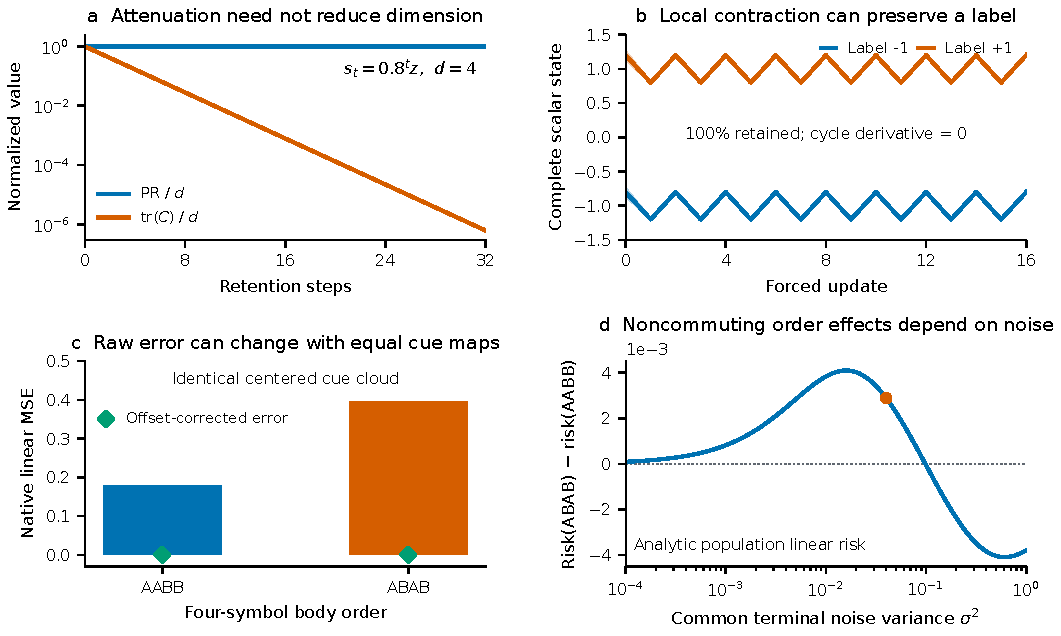
\includegraphics[width=\linewidth]{figures/analytic_controls.pdf}
\caption{\textbf{Diagnostic dissociations in constructed systems.}
(a) $s_t=0.8^t z$, with isotropic four-dimensional cues: normalized variance
decays while normalized PR remains one.
(b) Two phase-forced cubic attractors retain their labels; shaded envelopes
vary the initial perturbation by at most 0.05 and are not confidence intervals.
(c) Different affine offsets change native error while the cue map is unchanged;
offset correction removes the error.
(d) For two noncommuting matrices and matched symbol counts, the population
linear-risk difference between ABAB and AABB changes sign as common terminal
noise varies. The orange point uses noise covariance $0.04I$. These short
analytic bodies do not satisfy the full motif-matching design.}
\label{fig:controls}
\end{figure}

\subsection{The trained pilots fail the prerequisite for harmful-loss inference}
Four GRU/LSTM categorical/continuous pilots completed 1,500 optimization steps,
with one training seed (0) per cell and validation-selected checkpoints.
Saved predictions, complete-state arrays and compact reductions were independently
verified. Each behavior estimate uses 256 paired held-out episodes per horizon;
these episodes do not replace independent training seeds.
\Cref{fig:pilot-audit} shows the decisive outcome: all four cells fail even the
original engineering criterion at $R=1,2$, before the stricter research criterion.
Both categorical models achieve 5.47\%, 6.25\% and 5.08\% accuracy at
$R=1,2,16$ in both arms, against 6.25\% chance.
Continuous MSE is 0.998--1.018 times the exact saved-target zero-predictor MSE.
Periodic-minus-control MSE contrasts are at most $1.20\times10^{-7}$ in
magnitude. These near-zero contrasts cannot establish equivalence of competent
memory mechanisms.

\begin{figure}[t]
\centering
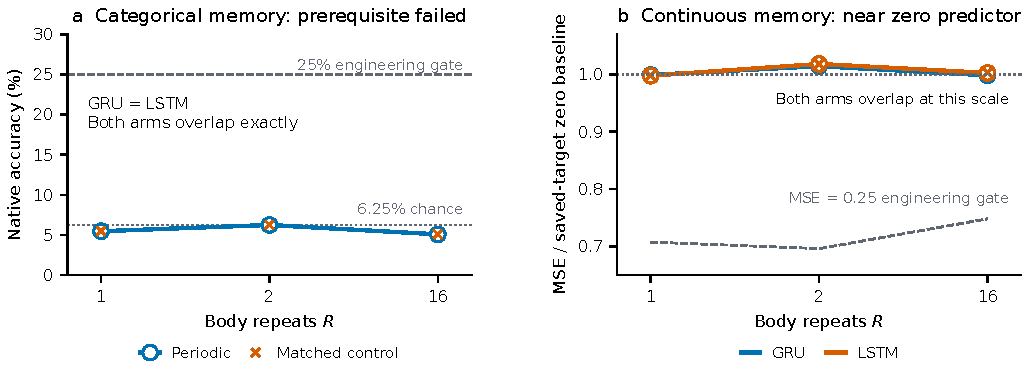
\includegraphics[width=\linewidth]{figures/pilot_audit.pdf}
\caption{\textbf{Native competence is absent in the verified seed-0 pilots.}
(a) The categorical GRU and LSTM have identical aggregate accuracies;
periodic circles and control crosses coincide exactly.
(b) Continuous errors are normalized by the zero-predictor error on the same
targets. Color denotes architecture; circles/crosses denote periodic/control
arms, which overlap at this display scale. Dashed lines show the original
25\% accuracy and 0.25 MSE engineering gates. No training-seed uncertainty
is estimated from a single fit per cell.}
\label{fig:pilot-audit}
\label{fig:pilots}
\end{figure}

\paragraph{Residual decodability qualifies the failure.}
At $R=2$, every cue-conditioned cloud has a held-out real-label probe advantage
over its shuffled-label control. Categorical probe accuracy spans
20.95--22.75\% for GRU and 14.75--15.53\% for LSTM; these ranges describe
four fixed-driver/arm clouds per cell, not uncertainty intervals.
Thus poor native behavior does not imply that all cue information is absent.
The $R=16$ probe advantages are inconsistent, but interpreting this difference
requires care: feature standardization uses a $10^{-8}$ floor, and the observed
state variations approach float32 coordinate spacing.
\Cref{app:probe-scale} gives an exact invertible-encoding counterexample in which
that floor alone makes ridge error approach the zero-predictor baseline.
It diagnoses a possible measurement confound without attributing the pilot
contrast to that confound. Full cloud measurements appear in
\cref{app:pilot-details}.

\paragraph{What the evidence licenses.}
The pilots establish failed native competence under this training protocol.
They do not localize the failure to acquisition, retention or readout, and
neither support nor falsify harmful periodic memory loss in competent models.
Independent checkpoint-only reduction verifies attenuation in both arms, with
precision-sensitive nonzero cue separation. Twenty subsequent local fits fail
full-coordinate competence before any distractor body, despite partial successes.
Twelve separate singleton-query fits pass at addresses 7 and 15 and fail at
address 0 (\cref{app:acquisition}); those different weights do not establish
joint eight-address recall. Acquisition, native readout and the causes of the
address-dependent pattern remain unresolved.
